% Generated by code/needham.py -- do not edit by hand.
\definecolor{qocA}{rgb}{0.00,0.45,0.70}
\definecolor{qocB}{rgb}{0.90,0.60,0.00}
\definecolor{qocC}{rgb}{0.00,0.62,0.45}
\definecolor{qocD}{rgb}{0.80,0.40,0.00}
\definecolor{qocE}{rgb}{0.80,0.60,0.70}
\definecolor{qocF}{rgb}{0.35,0.70,0.90}
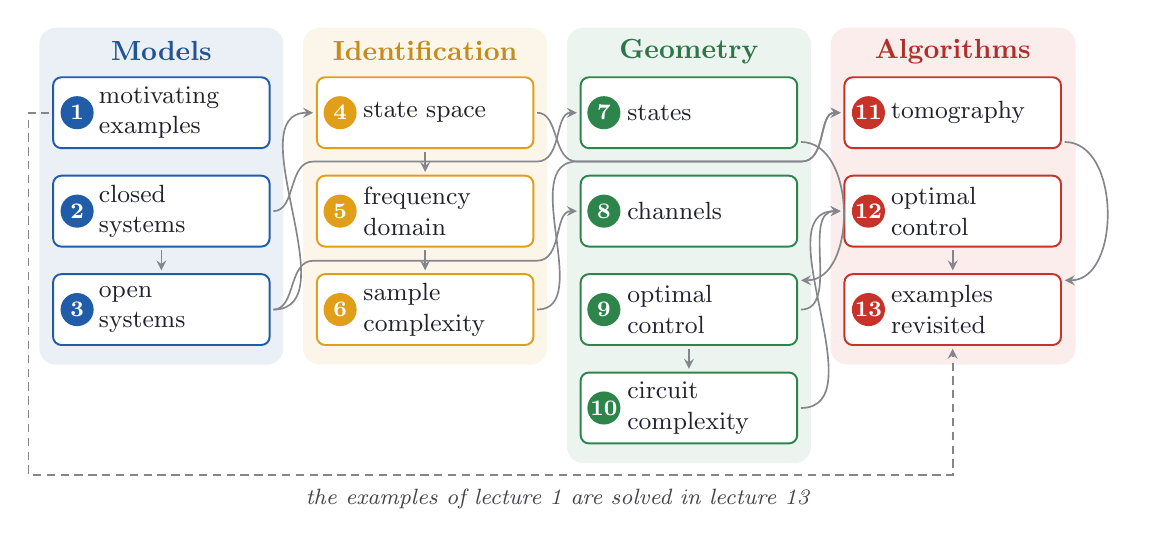
\begin{tikzpicture}[ink/.style={line width=0.9pt, ndInk}, faint/.style={line width=0.4pt, ndInk!35}, dashedink/.style={line width=0.5pt, ndInk!55, dash pattern=on 2.5pt off 2pt}, vec/.style={->, >=stealth, line width=1.2pt}, note/.style={font=\footnotesize\itshape, text=ndInk!85, align=center}, pointer/.style={->, >=stealth, line width=0.4pt, ndInk!60, shorten >=2pt, shorten <=1pt}, dot/.style={circle, fill=ndInk, inner sep=0pt, minimum size=3.4pt}, wash/.style={fill=ndSky, fill opacity=0.55}, every node/.style={text=ndInk}]
\definecolor{ndInk}{rgb}{0.13,0.13,0.18}
\definecolor{ndPaper}{rgb}{0.99,0.96,0.88}
\definecolor{ndSky}{rgb}{0.84,0.91,0.98}
\definecolor{ndRose}{rgb}{0.98,0.86,0.84}
\definecolor{ndBlue}{rgb}{0.13,0.36,0.66}
\definecolor{ndRed}{rgb}{0.78,0.20,0.16}
\definecolor{ndGold}{rgb}{0.88,0.62,0.10}
\definecolor{ndGreen}{rgb}{0.18,0.52,0.30}
\fill[ndBlue!9, rounded corners=6pt] (-1.55,-3.20) rectangle (1.55,1.08);
\node[font=\bfseries, text=ndBlue!85!ndInk] at (0.00,0.78) {Models};
\node[draw=ndBlue, line width=0.7pt, rounded corners=3pt, fill=white, minimum width=2.75cm, minimum height=0.90cm, inner sep=1pt] (L1) at (0.00,-0.00) {};
\node[circle, fill=ndBlue, text=white, font=\footnotesize\bfseries, inner sep=0pt, minimum size=0.42cm] at (-1.07,-0.00) {1};
\node[font=\small, anchor=west, align=left, inner sep=0pt] at (-0.80,-0.00) {motivating\\examples};
\node[draw=ndBlue, line width=0.7pt, rounded corners=3pt, fill=white, minimum width=2.75cm, minimum height=0.90cm, inner sep=1pt] (L2) at (0.00,-1.25) {};
\node[circle, fill=ndBlue, text=white, font=\footnotesize\bfseries, inner sep=0pt, minimum size=0.42cm] at (-1.07,-1.25) {2};
\node[font=\small, anchor=west, align=left, inner sep=0pt] at (-0.80,-1.25) {closed\\systems};
\node[draw=ndBlue, line width=0.7pt, rounded corners=3pt, fill=white, minimum width=2.75cm, minimum height=0.90cm, inner sep=1pt] (L3) at (0.00,-2.50) {};
\node[circle, fill=ndBlue, text=white, font=\footnotesize\bfseries, inner sep=0pt, minimum size=0.42cm] at (-1.07,-2.50) {3};
\node[font=\small, anchor=west, align=left, inner sep=0pt] at (-0.80,-2.50) {open\\systems};
\fill[ndGold!9, rounded corners=6pt] (1.80,-3.20) rectangle (4.90,1.08);
\node[font=\bfseries, text=ndGold!85!ndInk] at (3.35,0.78) {Identification};
\node[draw=ndGold, line width=0.7pt, rounded corners=3pt, fill=white, minimum width=2.75cm, minimum height=0.90cm, inner sep=1pt] (L4) at (3.35,-0.00) {};
\node[circle, fill=ndGold, text=white, font=\footnotesize\bfseries, inner sep=0pt, minimum size=0.42cm] at (2.27,-0.00) {4};
\node[font=\small, anchor=west, align=left, inner sep=0pt] at (2.56,-0.00) {state space};
\node[draw=ndGold, line width=0.7pt, rounded corners=3pt, fill=white, minimum width=2.75cm, minimum height=0.90cm, inner sep=1pt] (L5) at (3.35,-1.25) {};
\node[circle, fill=ndGold, text=white, font=\footnotesize\bfseries, inner sep=0pt, minimum size=0.42cm] at (2.27,-1.25) {5};
\node[font=\small, anchor=west, align=left, inner sep=0pt] at (2.56,-1.25) {frequency\\domain};
\node[draw=ndGold, line width=0.7pt, rounded corners=3pt, fill=white, minimum width=2.75cm, minimum height=0.90cm, inner sep=1pt] (L6) at (3.35,-2.50) {};
\node[circle, fill=ndGold, text=white, font=\footnotesize\bfseries, inner sep=0pt, minimum size=0.42cm] at (2.27,-2.50) {6};
\node[font=\small, anchor=west, align=left, inner sep=0pt] at (2.56,-2.50) {sample\\complexity};
\fill[ndGreen!9, rounded corners=6pt] (5.15,-4.45) rectangle (8.25,1.08);
\node[font=\bfseries, text=ndGreen!85!ndInk] at (6.70,0.78) {Geometry};
\node[draw=ndGreen, line width=0.7pt, rounded corners=3pt, fill=white, minimum width=2.75cm, minimum height=0.90cm, inner sep=1pt] (L7) at (6.70,-0.00) {};
\node[circle, fill=ndGreen, text=white, font=\footnotesize\bfseries, inner sep=0pt, minimum size=0.42cm] at (5.62,-0.00) {7};
\node[font=\small, anchor=west, align=left, inner sep=0pt] at (5.91,-0.00) {states};
\node[draw=ndGreen, line width=0.7pt, rounded corners=3pt, fill=white, minimum width=2.75cm, minimum height=0.90cm, inner sep=1pt] (L8) at (6.70,-1.25) {};
\node[circle, fill=ndGreen, text=white, font=\footnotesize\bfseries, inner sep=0pt, minimum size=0.42cm] at (5.62,-1.25) {8};
\node[font=\small, anchor=west, align=left, inner sep=0pt] at (5.91,-1.25) {channels};
\node[draw=ndGreen, line width=0.7pt, rounded corners=3pt, fill=white, minimum width=2.75cm, minimum height=0.90cm, inner sep=1pt] (L9) at (6.70,-2.50) {};
\node[circle, fill=ndGreen, text=white, font=\footnotesize\bfseries, inner sep=0pt, minimum size=0.42cm] at (5.62,-2.50) {9};
\node[font=\small, anchor=west, align=left, inner sep=0pt] at (5.91,-2.50) {optimal\\control};
\node[draw=ndGreen, line width=0.7pt, rounded corners=3pt, fill=white, minimum width=2.75cm, minimum height=0.90cm, inner sep=1pt] (L10) at (6.70,-3.75) {};
\node[circle, fill=ndGreen, text=white, font=\footnotesize\bfseries, inner sep=0pt, minimum size=0.42cm] at (5.62,-3.75) {10};
\node[font=\small, anchor=west, align=left, inner sep=0pt] at (5.91,-3.75) {circuit\\complexity};
\fill[ndRed!9, rounded corners=6pt] (8.50,-3.20) rectangle (11.61,1.08);
\node[font=\bfseries, text=ndRed!85!ndInk] at (10.05,0.78) {Algorithms};
\node[draw=ndRed, line width=0.7pt, rounded corners=3pt, fill=white, minimum width=2.75cm, minimum height=0.90cm, inner sep=1pt] (L11) at (10.05,-0.00) {};
\node[circle, fill=ndRed, text=white, font=\footnotesize\bfseries, inner sep=0pt, minimum size=0.42cm] at (8.98,-0.00) {11};
\node[font=\small, anchor=west, align=left, inner sep=0pt] at (9.26,-0.00) {tomography};
\node[draw=ndRed, line width=0.7pt, rounded corners=3pt, fill=white, minimum width=2.75cm, minimum height=0.90cm, inner sep=1pt] (L12) at (10.05,-1.25) {};
\node[circle, fill=ndRed, text=white, font=\footnotesize\bfseries, inner sep=0pt, minimum size=0.42cm] at (8.98,-1.25) {12};
\node[font=\small, anchor=west, align=left, inner sep=0pt] at (9.26,-1.25) {optimal\\control};
\node[draw=ndRed, line width=0.7pt, rounded corners=3pt, fill=white, minimum width=2.75cm, minimum height=0.90cm, inner sep=1pt] (L13) at (10.05,-2.50) {};
\node[circle, fill=ndRed, text=white, font=\footnotesize\bfseries, inner sep=0pt, minimum size=0.42cm] at (8.98,-2.50) {13};
\node[font=\small, anchor=west, align=left, inner sep=0pt] at (9.26,-2.50) {examples\\revisited};
\draw[->, >=stealth, line width=0.6pt, ndInk!55, shorten >=1pt, shorten <=1pt] (L2.south) -- (L3.north);
\draw[->, >=stealth, line width=0.6pt, ndInk!55, shorten >=1pt, shorten <=1pt] (L3.east) to[out=0, in=180] (L4.west);
\draw[->, >=stealth, line width=0.6pt, ndInk!55, shorten >=1pt, shorten <=1pt] (L4.south) -- (L5.north);
\draw[->, >=stealth, line width=0.6pt, ndInk!55, shorten >=1pt, shorten <=1pt] (L5.south) -- (L6.north);
\draw[->, >=stealth, line width=0.6pt, ndInk!55, shorten >=1pt, shorten <=1pt] (L2.east) to[out=0, in=180] (1.93,-0.62) -- (4.77,-0.62) to[out=0, in=180] (L7.west);
\draw[->, >=stealth, line width=0.6pt, ndInk!55, shorten >=1pt, shorten <=1pt] (L3.east) to[out=0, in=180] (1.93,-1.88) -- (4.77,-1.88) to[out=0, in=180] (L8.west);
\draw[->, >=stealth, line width=0.6pt, ndInk!55, shorten >=1pt, shorten <=1pt] (L7.345) .. controls +(0.75,0) and +(0.75,0) .. (L9.15);
\draw[->, >=stealth, line width=0.6pt, ndInk!55, shorten >=1pt, shorten <=1pt] (L9.south) -- (L10.north);
\draw[->, >=stealth, line width=0.6pt, ndInk!55, shorten >=1pt, shorten <=1pt] (L6.east) to[out=0, in=180] (5.28,-0.62) -- (8.13,-0.62) to[out=0, in=180] (L11.west);
\draw[->, >=stealth, line width=0.6pt, ndInk!55, shorten >=1pt, shorten <=1pt] (L4.east) to[out=0, in=180] (5.28,-0.62) -- (8.13,-0.62) to[out=0, in=180] (L11.west);
\draw[->, >=stealth, line width=0.6pt, ndInk!55, shorten >=1pt, shorten <=1pt] (L9.east) to[out=0, in=180] (L12.west);
\draw[->, >=stealth, line width=0.6pt, ndInk!55, shorten >=1pt, shorten <=1pt] (L10.east) to[out=0, in=180] (L12.west);
\draw[->, >=stealth, line width=0.6pt, ndInk!55, shorten >=1pt, shorten <=1pt] (L11.345) .. controls +(0.75,0) and +(0.75,0) .. (L13.15);
\draw[->, >=stealth, line width=0.6pt, ndInk!55, shorten >=1pt, shorten <=1pt] (L12.south) -- (L13.north);
\draw[->, >=stealth, line width=0.6pt, ndInk!55, shorten >=1pt, shorten <=1pt, dash pattern=on 3pt off 2pt] (L1.west) -- ++(-0.3,0) |- (9.45,-4.60) -| (L13.south);
\node[note, anchor=north] at (5.03,-4.65) {the examples of lecture 1 are solved in lecture 13};
\end{tikzpicture}
